\section{Lecture 7 (10 IV 2019)}
\begin{figure}[H]
    \centering
    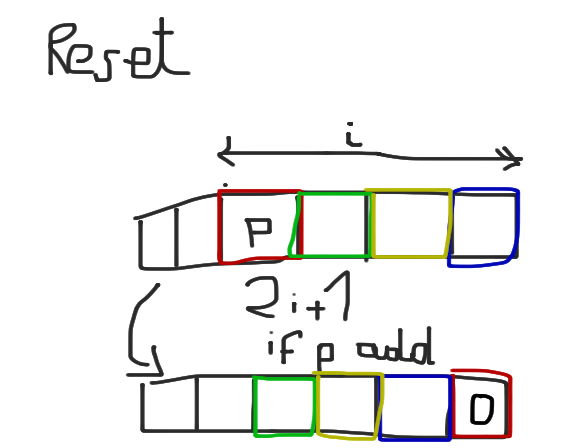
\includegraphics[scale=0.2]{content/graphics/game7.png}
\end{figure}
Parity games $n$, $\underbrace{d}_{rank}$.\\

\noindent
Karoliina Lehtinen -- algorithm.\\
$G$ -- a finite parity game.\\
We create a game $\mathcal{R}^E_k(G)$ with $k$ registers containing priorities $Mem \subseteq \{0, 1, ..., d\}^k$.
$\widetilde{Pos_E} = (Pos \times Mem \times \{0\}) \cup (Pos_E \times Mem \times \{1\})$\\
$\widetilde{Pos_A} = Pos_A \times Mem \times \{1\}$.\\

\noindent
If $p \rightarrow q$ in $G$ then\\
$(p, \alpha, 1) \xrightarrow[\text{1}] (q, up(\alpha), 0)$\\
$(p, \alpha, 0) \rightarrow (p, reset(\alpha), 1)$\\
$(p, \alpha, 0) \xrightarrow[\text{1}]{\text{[skip]}} (p, \alpha, 1)$\\

\noindent
$[up(\alpha)]_i = max(\alpha_i, rank(q))$\\

\noindent
\textbf{Lemma 1} If Adam wins original game $G$ from position $p$,
he wins $\mathcal{R}^E_k(G)$ from position $(p, \alpha, 1)$ for any number of registers $k$.\\
Adam plays the strategy from original game, we will show that any play is winning. Let $q$ be the maximal odd rank.
Let $i$ be the deepest register, which resets infinitely often. We will show, that infinitely often,
in the moment of reset of the register $i$, it contains $q$.\\

\noindent
\textbf{Lemma 2} If Eve wins the game $G$ from position $p$,
then $(\exists_k)$ Eve wins $\mathcal{R}^E_k(G)$ from position $(p, \alpha, 0)$.\\
$k$: number of ranks from the original game.\\
To each even rank $d$ we dedicate some register. When in original game there appears
an odd rank $d$, Eve resets the register dedicated to rank $d$.